\documentclass[conference]{IEEEtran}
\usepackage{graphicx,booktabs,amsmath,url}
\newcommand{\todo}[1]{\textbf{[TODO: #1]}}

\begin{document}
\title{CNNs, Vision Transformers and Pretrained Features for RIVAL10 Image Classification}
\author{\IEEEauthorblockN{\todo{Names, alphabetical}}\IEEEauthorblockA{ECSE 551, McGill University, Fall 2026}}
\maketitle

\begin{abstract}
We study 10-class image classification on RIVAL10, an ImageNet-derived dataset with object masks. For Task~1 we design and train from scratch a 3-layer convolutional neural network (CNN) and a vision transformer (ViT). Design choices for the CNN were made by a controlled ablation: each change was tested with two seeds on a fixed validation split and kept only if it improved accuracy. We compare the two models beyond accuracy, with per-class results, a contingency table of joint correct/incorrect predictions, and mask-based tests of whether each model relies on the object or on the background. For Task~2 we use frozen features from three pretrained backbones (DINOv2, SigLIP2, ConvNeXt) with linear probes and a probability-averaging ensemble. The CNN reaches 84.2\,\% on our held-out test split, and the Task~2 ensemble 99.8\,\% (Kaggle public score 0.998). \todo{ViT number}
\end{abstract}

\section{Introduction}
The assignment has two tasks: (1) design, train from scratch and analyse a CNN and a ViT; (2) obtain the best possible accuracy with any method, including pretrained models. Both are evaluated on a Kaggle competition. \todo{most important findings, 2--3 sentences}

\section{Methodology}
\subsection{CNN}
\textbf{Baseline.} The baseline is a single $11\times11$ convolution (96 filters, stride 4), ReLU, max-pooling and a linear layer on the flattened feature maps, trained with Adam ($\text{lr}=10^{-3}$).

\textbf{Architecture.} The final model stacks three blocks of $3\times3$ convolution $\rightarrow$ batch normalization $\rightarrow$ ReLU $\rightarrow$ $2\times2$ max-pooling, with $w$, $2w$ and $4w$ filters. Stacking small kernels lets each layer see a larger area than the one before: the first layer finds edges, the next ones textures and object parts. This needs fewer parameters than one large kernel, and each pooling halves the resolution so deeper filters see more of the image. Batch normalization stabilizes the activations, which permits higher learning rates. A global average pooling layer reduces each of the $4w$ maps to one number before a dropout layer and a linear classifier. This needs far fewer weights than flattening, which limits overfitting.

\textbf{Training.} We use the cross-entropy loss, the standard choice for single-label classification: it is the negative log-likelihood of the softmax output, so minimizing it pushes up the probability of the correct class. Label smoothing replaces the one-hot target by $0.9$ on the correct class and spreads $0.1$ over all classes, which discourages over-confident predictions. The optimizer is AdamW: Adam adapts the step size of each weight, so it works with little tuning, and AdamW applies weight decay directly to the weights, separately from the gradient step. We use a batch size of 128 and 30 (or 60) epochs. After each epoch we compute the validation accuracy and save the weights whenever it improves (\texttt{torch.save} of the \texttt{state\_dict}). The stopping criterion is therefore early stopping by model selection: the final model is the best-validation epoch, and all test predictions are made with these saved weights. The following components can be switched on or off and are tested in the ablation: (i) augmentation, implemented as one random affine transform per image (zoom keeping 75--100\,\% of the image, random translation, horizontal flip); (ii) regularization: weight decay $5\cdot10^{-4}$, label smoothing 0.1 and dropout 0.3; (iii) a OneCycle learning-rate schedule (warm-up, then cosine decay); (iv) test-time flip: the logits of the image and its mirror image are averaged. On the GPU we train in mixed precision (float16), which halves the training time.

\textbf{Hyperparameter selection.} We follow a one-factor-at-a-time protocol. Starting from the 3-layer CNN trained with the baseline's settings, we add one change at a time: augmentation, regularization and schedule, width $w=64$, resolution 112, test-time flip, 60 instead of 30 epochs, and finally augmentation again if it was rejected at the first step (a change can help only once training is long and regularized). Each change is trained with seeds 0 and 1 and kept only if the mean validation accuracy improves. Finally, the learning rate is chosen among $\{3\cdot10^{-4}, 10^{-3}, 3\cdot10^{-3}\}$. The test split is used once, for the final model. The selected configuration is: width $w=64$, $64\times64$ input, dropout 0.3, weight decay $5\cdot10^{-4}$, label smoothing 0.1, OneCycle schedule with maximum learning rate $3\cdot10^{-3}$, 60 epochs, test-time flip, and no augmentation (373{,}834 parameters).

\subsection{Vision Transformer}
\todo{ViT owner: patch embedding, [CLS] token, positional embedding, encoder blocks (pre-norm MHSA + MLP), head; training setup and hyperparameter selection}

\subsection{Analysis protocol (Task 1)}
\textbf{Comparison beyond accuracy.} Both models are evaluated on the same held-out test split. We report per-class accuracy and confusion matrices, and a $2\times2$ contingency table counting the images that both models classify correctly, only the CNN, only the ViT, and neither. McNemar's test on the two off-diagonal counts tells whether the difference between the models is statistically significant.

\textbf{What the models rely on.} Each image has a binary object mask, which we resize to the model's input resolution. On the test split we apply six conditions and measure overall and per-class accuracy: (i) clean; (ii) Gaussian noise ($\sigma=0.3$ on the $[0,1]$ pixel scale) on the object only; (iii) the same noise on the background only; (iv) background replaced by the mean training colour (object only); (v) object replaced by the mean colour (background only); (vi) object pasted onto the background of a random other test image, whose own object is blanked. A model that loses more accuracy under background noise than under object noise, or that stays well above chance (10\,\%) with the object removed, relies on the context around the object.

\subsection{Task 2: pretrained features}
We freeze three pretrained backbones, chosen because they were trained in very different ways, and use them as feature extractors: DINOv2-L with registers~\cite{dinov2} (self-supervised ViT, 304M parameters), SigLIP2 So400m~\cite{siglip2} (ViT trained on image--text pairs) and ConvNeXt-L~\cite{convnext} (CNN trained with labels on ImageNet-22k, then ImageNet-1k). Each image is embedded at $224\times224$, and the embedding is averaged with that of its horizontal flip (test-time augmentation) and $L_2$-normalized. A multinomial logistic regression is fitted per backbone, with its inverse regularization $C$ chosen on the validation split. The ensemble averages the class probabilities of a subset of the models. All seven subsets (each model alone, the three pairs, all three) are scored on the validation split and the best is kept, so the test split is never used for a choice. For the Kaggle predictions the chosen probes are refit on all labelled images; their weights, together with the names of the frozen public checkpoints, form the submitted Task~2 weights. Because RIVAL10 is drawn from ImageNet, the backbones' pretraining data may overlap with it, so these accuracies may overstate performance on truly new images; this is strongest for ConvNeXt, which saw ImageNet labels.

\section{Dataset}
RIVAL10~\cite{rival10} contains images from 20 ImageNet synsets grouped into 10 classes (truck, frog, cat, plane, bird, car, equine, ship, deer, dog). The provided training set has 21{,}098 labelled $224\times224$ RGB images with a balanced class distribution (2{,}011--2{,}127 per class), and the test set has 5{,}286 unlabelled images. Each image comes with a binary object mask. We split the labelled data once into 70\,\% training, 15\,\% validation and 15\,\% test, stratified by class with a fixed seed (\texttt{split.csv}); all models use this split. Images are normalized per channel with the training-split mean and standard deviation. For the from-scratch models they are downsampled (antialiased bilinear) to $64\times64$ or $112\times112$, which we treat as a hyperparameter.

\section{Results}
\subsection{CNN ablation}
Table~\ref{tab:ablation} lists every step of the ablation. Replacing the single large convolution by three small-kernel blocks gives the largest jump (+13.0 points), so on this dataset several small filters learn better features than one big filter. Regularization (+1.7), a wider network (+4.4) and test-time flip (+0.5) each helped. Training for 60 instead of 30 epochs gave +4.3 points: with regularization and the OneCycle schedule, the model keeps improving for longer. The learning-rate sweep (one seed each) chose $3\cdot10^{-3}$ (0.855, against 0.827 for $10^{-3}$ and 0.766 for $3\cdot10^{-4}$); batch normalization makes such a high rate stable.

Two changes were rejected. Increasing the resolution to $112\times112$ lowered accuracy by 1.0 point. With three $3\times3$ convolutions and three poolings, each output unit sees a $22\times22$-pixel window. At $64\times64$ this covers a third of the image; at $112\times112$ only a fifth, so the network sees a smaller part of the object for the same depth. Augmentation was rejected twice: at the first step ($-2.8$ points) and again on the final setup ($-4.1$ points). Augmentation makes the training task harder. With 374k parameters and 60 epochs, the model does not have the time or capacity to benefit from it, even though the learning curves (Fig.~\ref{fig:curves}) show overfitting: training accuracy reaches 97\,\% while validation accuracy levels off at 85\,\%. A longer schedule or a deeper network would probably be needed for augmentation to pay off.

\begin{table}[t]
\centering
\caption{CNN ablation: validation accuracy, mean and standard deviation over seeds 0 and 1. Each step adds one change to the best configuration so far.}
\label{tab:ablation}
\begin{tabular}{lccl}
\toprule
Step & Val acc & Std & Decision \\
\midrule
Baseline (1 conv layer) & 0.5869 & 0.0043 & reference \\
3-layer CNN & 0.7166 & 0.0009 & start \\
+ augmentation & 0.6889 & 0.0216 & rejected \\
+ regularization + OneCycle & 0.7338 & 0.0039 & kept \\
Width 64 & 0.7777 & 0.0008 & kept \\
Resolution 112 & 0.7678 & 0.0019 & rejected \\
+ test-time flip & 0.7826 & 0.0032 & kept \\
60 epochs & 0.8253 & 0.0022 & kept \\
+ augmentation (retest) & 0.7839 & 0.0041 & rejected \\
Learning rate $3\cdot10^{-3}$ & 0.8550 & -- & kept (1 seed) \\
\bottomrule
\end{tabular}
\end{table}

\begin{figure}[t]
\centering
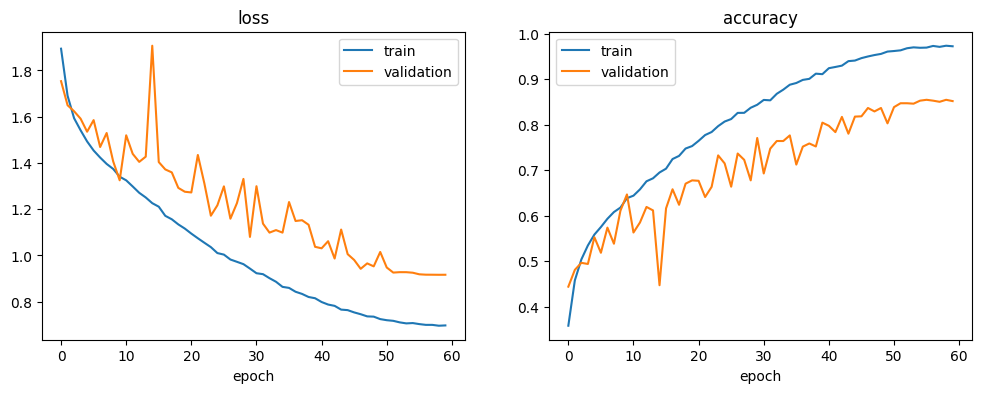
\includegraphics[width=\columnwidth]{figures/cnn_curves.png}
\caption{Learning curves of the final CNN. The gap between training and validation accuracy shows overfitting; validation accuracy stops improving as the learning rate decays to zero.}
\label{fig:curves}
\end{figure}

\subsection{Final models: train / validation / test}
\begin{table}[t]
\centering
\caption{Final models on our train / validation / test split.}
\label{tab:final}
\begin{tabular}{lccccc}
\toprule
Model & Params & Train & Val & Test & Kaggle \\
\midrule
CNN & 374k & 0.9632 & 0.8550 & 0.8417 & \todo{} \\
ViT & \todo{} & \todo{} & \todo{} & \todo{} & \todo{} \\
\bottomrule
\end{tabular}
\end{table}

The CNN reaches 84.2\,\% on our test split, close to its 85.5\,\% validation accuracy, so choosing the settings on the validation split did not make it optimistic by much. The 12-point gap to the training accuracy is the overfitting discussed above.

\subsection{Beyond accuracy}
The CNN's per-class test accuracy ranges from 78.0\,\% (dog) to 88.4\,\% (ship). Its confusion matrix (Fig.~\ref{fig:conf}) shows that most errors are between classes that look alike: cat and dog are confused in both directions (10\,\% each), truck is taken for car (8\,\%), bird for frog and equine for deer (6\,\% each). Vehicles with a distinctive shape and background (plane, ship, car) are recognized best. \todo{ViT per-class results; contingency table and McNemar test}

\begin{figure}[t]
\centering
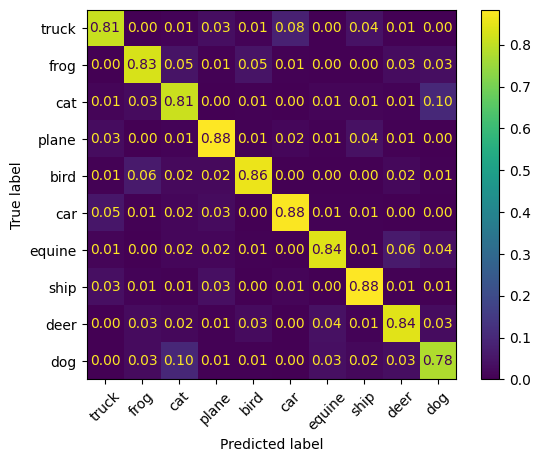
\includegraphics[width=0.85\columnwidth]{figures/cnn_confusion.png}
\caption{CNN confusion matrix on our test split (rows normalized: each row sums to 1).}
\label{fig:conf}
\end{figure}

\subsection{What do the models look at?}
Table~\ref{tab:masks} shows the CNN's accuracy under the six mask conditions. The object covers 37\,\% of the pixels on average.

\textbf{The background alone is informative.} With the object blanked, the CNN still reaches 31.1\,\%, three times chance (10\,\%). This comes from a few classes: plane (82.9\,\%) and bird (79.0\,\%) are most likely recognized from the sky, ship (46.5\,\%) from the water and deer (46.1\,\%) from the forest. Car, cat and dog fall to 2--4\,\%: for these the network needs the object. With the background blanked (object only), accuracy is 42.9\,\%. Plane and bird stay high, which is consistent with a uniform grey fill looking like sky to the network. Pasting the object onto another image's background gives 44.6\,\%, so a misleading background costs about 40 points.

\textbf{Noise.} Gaussian noise with $\sigma=0.3$ is too strong for a model that never saw noise in training: accuracy falls to 27\,\% whether the noise is on the object or on the background. Some classes keep a high accuracy under noise (cat 90.6\,\% with background noise, plane 88.6\,\% with object noise), which suggests the model tends to predict these classes for noisy images in general, so the per-class numbers under noise should be read with care. A sweep over smaller $\sigma$ would separate the two cases better.

The CNN uses the object for classes defined by their shape (car, cat, dog). For classes with a typical background (plane, bird, ship, deer), it relies heavily on that background. This shortcut explains part of its errors and would hurt on images with unusual backgrounds. \todo{same analysis for the ViT}

\begin{table}[t]
\centering
\caption{CNN test accuracy when only the object or only the background is modified (overall and selected classes).}
\label{tab:masks}
\begin{tabular}{lcccccc}
\toprule
Condition & All & Plane & Bird & Ship & Car & Dog \\
\midrule
Clean & 0.842 & 0.883 & 0.859 & 0.884 & 0.878 & 0.780 \\
Noise on object & 0.269 & 0.886 & 0.455 & 0.066 & 0.000 & 0.104 \\
Noise on background & 0.276 & 0.117 & 0.100 & 0.270 & 0.094 & 0.538 \\
Background blanked & 0.429 & 0.943 & 0.859 & 0.242 & 0.558 & 0.311 \\
Object blanked & 0.311 & 0.829 & 0.790 & 0.465 & 0.016 & 0.035 \\
Background swapped & 0.446 & 0.775 & 0.668 & 0.236 & 0.683 & 0.362 \\
\bottomrule
\end{tabular}
\end{table}

\subsection{Task 2}
Table~\ref{tab:task2} shows the accuracy of every subset of probes. All backbones are above 99.6\,\% on their own. DINOv2 + ConvNeXt has the best validation accuracy (2 errors out of 3{,}165 images) and was chosen ($C=10$ and $C=3$). On our test split it makes 7 errors (99.78\,\%). The subsets differ by only 1--3 images, so they are practically equivalent. On the Kaggle leaderboard it reaches a public score of 0.99810.

\begin{table}[t]
\centering
\caption{Task 2: accuracy of each probe subset (mean of probabilities).}
\label{tab:task2}
\begin{tabular}{lcc}
\toprule
Models & Val acc & Test acc \\
\midrule
DINOv2 & 0.9981 & 0.9968 \\
SigLIP2 & 0.9987 & 0.9975 \\
ConvNeXt & 0.9987 & 0.9981 \\
DINOv2 + SigLIP2 & 0.9981 & 0.9975 \\
\textbf{DINOv2 + ConvNeXt (chosen)} & \textbf{0.9994} & 0.9978 \\
SigLIP2 + ConvNeXt & 0.9991 & 0.9981 \\
All three & 0.9991 & 0.9981 \\
\bottomrule
\end{tabular}
\end{table}

\section{Discussion and Conclusion}
\todo{Key findings; CNN inductive bias vs ViT data hunger; future work}

\section*{Statement of Contributions}
\todo{Who did what}

\begin{thebibliography}{9}
\bibitem{rival10} M.~Moayeri, P.~Pope, Y.~Balaji, and S.~Feizi, ``A comprehensive study of image classification model sensitivity to foregrounds, backgrounds, and visual attributes,'' in \emph{Proc. CVPR}, 2022.
\bibitem{dinov2} M.~Oquab \emph{et al.}, ``DINOv2: Learning robust visual features without supervision,'' \emph{TMLR}, 2024.
\bibitem{siglip2} M.~Tschannen \emph{et al.}, ``SigLIP 2: Multilingual vision-language encoders with improved semantic understanding, localization, and dense features,'' arXiv:2502.14786, 2025.
\bibitem{convnext} Z.~Liu \emph{et al.}, ``A ConvNet for the 2020s,'' in \emph{Proc. CVPR}, 2022.
\end{thebibliography}
\end{document}
